\documentclass{article}

\usepackage{Sweave}
\begin{document}
\Sconcordance{concordance:regressionpdf.tex:regressionpdf.Rnw:%
1 2 1 1 0 5 1 1 2 1 0 2 1 1 6 10 0 1 3 3 1}


\emph{Vardan and Fez}


\begin{Schunk}
\begin{Sinput}
> library("ggplot2")
> ndata <- read.csv("AAPL SPX 10Y OiL - Copy.csv")
> attach(ndata)
> ##testing the creation of PDF
> ggplot(ndata,aes(y=aapl,x=spx))+geom_point(mapping = NULL)+stat_summary(fun.data=mean_cl_normal) + 
+   geom_smooth(method='lm',formula=aapl~spx)+theme_bw() +
+   labs(y = "AAPL",
+        x = "SPX",
+        title = "Regression Line")
> 
\end{Sinput}
\end{Schunk}
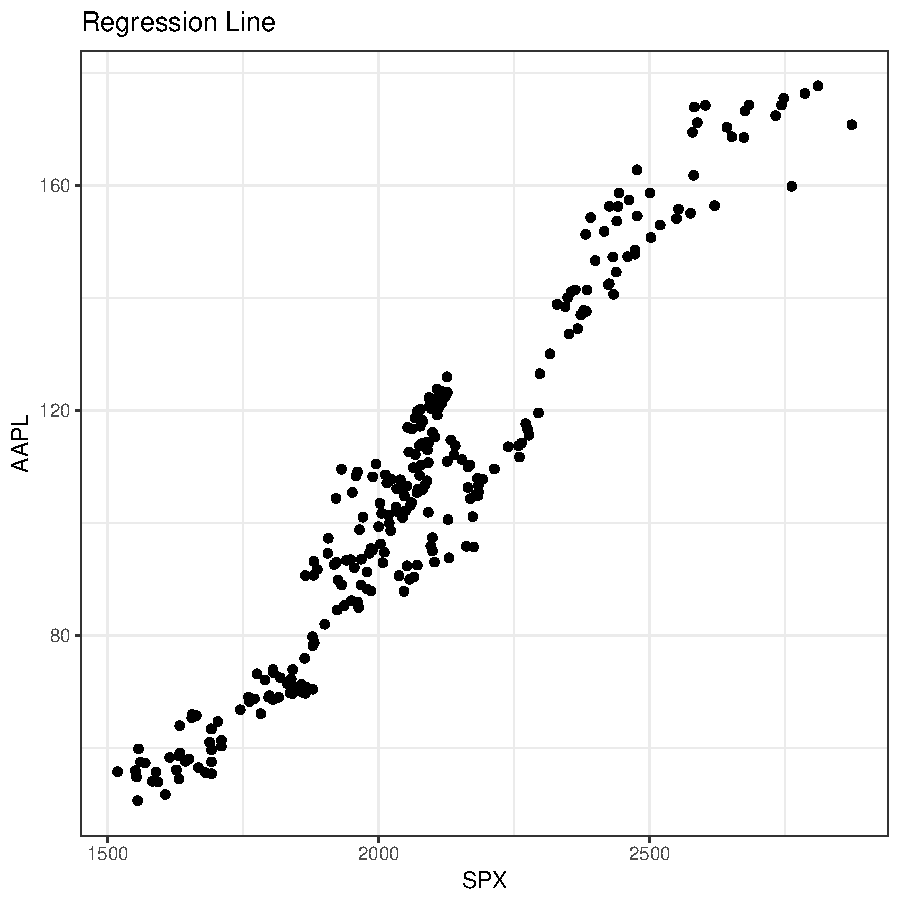
\includegraphics{regressionpdf-001}



\end{document}
